\documentclass[]{article}
\usepackage{lmodern}
\usepackage{amssymb,amsmath}
\usepackage{ifxetex,ifluatex}
\usepackage{fixltx2e} % provides \textsubscript
\ifnum 0\ifxetex 1\fi\ifluatex 1\fi=0 % if pdftex
  \usepackage[T1]{fontenc}
  \usepackage[utf8]{inputenc}
\else % if luatex or xelatex
  \ifxetex
    \usepackage{mathspec}
  \else
    \usepackage{fontspec}
  \fi
  \defaultfontfeatures{Ligatures=TeX,Scale=MatchLowercase}
\fi
% use upquote if available, for straight quotes in verbatim environments
\IfFileExists{upquote.sty}{\usepackage{upquote}}{}
% use microtype if available
\IfFileExists{microtype.sty}{%
\usepackage{microtype}
\UseMicrotypeSet[protrusion]{basicmath} % disable protrusion for tt fonts
}{}
\usepackage[margin=1in]{geometry}
\usepackage{hyperref}
\hypersetup{unicode=true,
            pdftitle={PHC410 (PHARMACEUTICAL BIOSTATISTICS)  Descriptive Statistics},
            pdfauthor={Dr Yuslina Zakaria},
            pdfborder={0 0 0},
            breaklinks=true}
\urlstyle{same}  % don't use monospace font for urls
\usepackage{graphicx,grffile}
\makeatletter
\def\maxwidth{\ifdim\Gin@nat@width>\linewidth\linewidth\else\Gin@nat@width\fi}
\def\maxheight{\ifdim\Gin@nat@height>\textheight\textheight\else\Gin@nat@height\fi}
\makeatother
% Scale images if necessary, so that they will not overflow the page
% margins by default, and it is still possible to overwrite the defaults
% using explicit options in \includegraphics[width, height, ...]{}
\setkeys{Gin}{width=\maxwidth,height=\maxheight,keepaspectratio}
\IfFileExists{parskip.sty}{%
\usepackage{parskip}
}{% else
\setlength{\parindent}{0pt}
\setlength{\parskip}{6pt plus 2pt minus 1pt}
}
\setlength{\emergencystretch}{3em}  % prevent overfull lines
\providecommand{\tightlist}{%
  \setlength{\itemsep}{0pt}\setlength{\parskip}{0pt}}
\setcounter{secnumdepth}{0}
% Redefines (sub)paragraphs to behave more like sections
\ifx\paragraph\undefined\else
\let\oldparagraph\paragraph
\renewcommand{\paragraph}[1]{\oldparagraph{#1}\mbox{}}
\fi
\ifx\subparagraph\undefined\else
\let\oldsubparagraph\subparagraph
\renewcommand{\subparagraph}[1]{\oldsubparagraph{#1}\mbox{}}
\fi

%%% Use protect on footnotes to avoid problems with footnotes in titles
\let\rmarkdownfootnote\footnote%
\def\footnote{\protect\rmarkdownfootnote}

%%% Change title format to be more compact
\usepackage{titling}

% Create subtitle command for use in maketitle
\providecommand{\subtitle}[1]{
  \posttitle{
    \begin{center}\large#1\end{center}
    }
}

\setlength{\droptitle}{-2em}

  \title{PHC410 (PHARMACEUTICAL BIOSTATISTICS) Descriptive Statistics}
    \pretitle{\vspace{\droptitle}\centering\huge}
  \posttitle{\par}
    \author{Dr Yuslina Zakaria}
    \preauthor{\centering\large\emph}
  \postauthor{\par}
      \predate{\centering\large\emph}
  \postdate{\par}
    \date{September 3, 2019}

\usepackage{booktabs}
\usepackage{longtable}
\usepackage{array}
\usepackage{multirow}
\usepackage{wrapfig}
\usepackage{float}
\usepackage{colortbl}
\usepackage{pdflscape}
\usepackage{tabu}
\usepackage{threeparttable}
\usepackage{threeparttablex}
\usepackage[normalem]{ulem}
\usepackage{makecell}
\usepackage{xcolor}

\begin{document}
\maketitle

\hypertarget{learning-outcomes}{%
\subsection{Learning Outcomes}\label{learning-outcomes}}

At the end of this lesson, students should be able to:

\begin{enumerate}
\def\labelenumi{\arabic{enumi}.}
\tightlist
\item
  differentiate all types of variables.
\item
  understand scale of measurements.
\item
  describe and calculate the properties of data.
\end{enumerate}

\hypertarget{outlines}{%
\subsection{Outlines}\label{outlines}}

\begin{itemize}
\tightlist
\item
  Introduction
\item
  Types of Variables
\item
  Scales of Measurements
\item
  Population \& Samples
\item
  Measures of Central Tendency
\item
  Measure of Dispersion
\item
  Properties of Distribution
\end{itemize}

\hypertarget{what-is-statistical-analysis}{%
\subsection{What is statistical
analysis?}\label{what-is-statistical-analysis}}

\begin{itemize}
\item
  Collection, analysis, interpretation and presentation of data to
  discover its underlying causes, patterns, relationships and trends.
\item
  Two major branches of statistics:

  \begin{enumerate}
  \def\labelenumi{\arabic{enumi}.}
  \tightlist
  \item
    Descriptive statistics
  \item
    Inferential statistics
  \end{enumerate}
\end{itemize}

\hypertarget{descriptive-statistics}{%
\subsection{Descriptive Statistics}\label{descriptive-statistics}}

\begin{itemize}
\tightlist
\item
  Procedures used to {\textbf{summarise and organise}} a set of scores
  or observations in a meaningful way.
\item
  Typically presented graphically, in tabular form (in tables), or as
  summary statistics (single values).
\item
  Descriptive statistics {\textbf{do not allow us to make conclusions}}
  beyond the data we have analysed or reach conclusions regarding any
  hypotheses we might have made.
\end{itemize}

\hypertarget{descriptive-statistics-cont.}{%
\subsection{Descriptive Statistics
(cont.)}\label{descriptive-statistics-cont.}}

\begin{itemize}
\tightlist
\item
  Allow simpler interpretation of data.
\item
  Used when the intent is to describe the data that they actually
  collected.
\item
  Example:

  \begin{itemize}
  \tightlist
  \item
    A clinical psychologist conducted a study in which she gave some of
    her clients a new depression treatment and she wanted to
    {\textbf{describe the average depression score}} of only those
    clients who got the treatment.
  \end{itemize}
\end{itemize}

\hypertarget{inferential-statistics}{%
\subsection{Inferential Statistics}\label{inferential-statistics}}

\begin{itemize}
\tightlist
\item
  Procedures that allow researchers {\textbf{to infer or generalize
  observations}} made with samples to the larger population from which
  they are selected.
\item
  Infer the value of population parameter from a sample statistics.
\item
  Determine the probability of characteristics of population based on
  the characteristics of the sample.
\end{itemize}

\hypertarget{inferential-statistics-cont.}{%
\subsection{Inferential Statistics
(cont.)}\label{inferential-statistics-cont.}}

\begin{itemize}
\tightlist
\item
  They help {\textbf{assess strength of the relationship}} between your
  independent (causal) variables, and your dependent (effect) variables.
\item
  Examples:

  \begin{itemize}
  \tightlist
  \item
    A clinical psychologist conducted a study in which she gave some of
    her clients a new depression treatment and she wanted to
    {\textbf{estimate}} what the results would be if she were to give
    the same treatment to additional clients.
  \end{itemize}
\end{itemize}

\hypertarget{statistical-analysis}{%
\subsection{Statistical analysis}\label{statistical-analysis}}

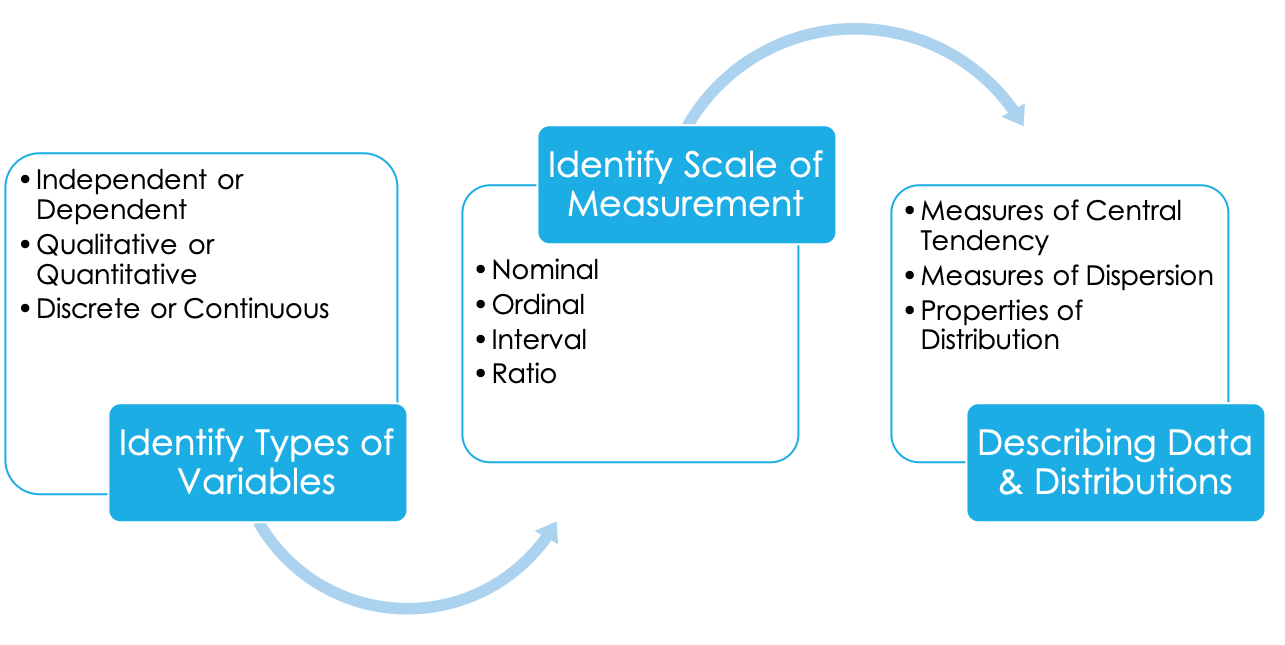
\includegraphics[width=1.05\linewidth]{figure/Ch1-Fig1}

\hypertarget{types-of-variables}{%
\subsection{Types of Variables}\label{types-of-variables}}

\begin{itemize}
\item
  Variables are measurements or observations that are typically numeric.
\item
  Three categories of variables:

  \begin{enumerate}
  \def\labelenumi{\arabic{enumi}.}
  \tightlist
  \item
    Independent VS Dependent
  \item
    Continuous VS Discrete
  \item
    Quantitative VS Qualitative
  \end{enumerate}
\end{itemize}

\hypertarget{independent-vs-dependent}{%
\subsection{Independent VS Dependent}\label{independent-vs-dependent}}

\begin{enumerate}
\def\labelenumi{\arabic{enumi}.}
\tightlist
\item
  Independent variable (IV)

  \begin{itemize}
  \tightlist
  \item
    Variable with two or more levels that are expected to {\textbf{have
    effects on another variable}}. (affect/change other outcome
    variable)
  \item
    Sometimes called as {\textbf{predictor}} or experimental variable.
  \end{itemize}
\item
  Dependent variable (DV)

  \begin{itemize}
  \tightlist
  \item
    The outcome variable that is used to {\textbf{compare the effects}}
    of the different independent variable (IV) levels.
  \end{itemize}
\end{enumerate}

\hypertarget{independent-vs-dependent-cont.}{%
\subsection{Independent VS Dependent
(cont.)}\label{independent-vs-dependent-cont.}}

\begin{itemize}
\tightlist
\item
  Example:
\end{itemize}

In an experiment to study the effects of a new treatment on reducing
depressive symptoms, researchers gave the new treatment to a sample of
people with depression and withhold the treatment from another sample of
people with depression. (i.e.~{\textbf{new treatment}} vs {\textbf{no
treatment}}). After both samples were given their respective treatment
levels, {\textbf{the amount of depression}} in each sample was compared
by counting the number of depressive symptoms.

\hypertarget{independent-vs-dependent-cont.-1}{%
\subsection{Independent VS Dependent
(cont.)}\label{independent-vs-dependent-cont.-1}}

\begin{enumerate}
\def\labelenumi{\arabic{enumi}.}
\tightlist
\item
  Independent variable (IV)

  \begin{itemize}
  \tightlist
  \item
    The new treatment
  \item
    No treatment
  \end{itemize}
\item
  Dependent variable (DV)

  \begin{itemize}
  \tightlist
  \item
    Amount of depression
  \end{itemize}
\end{enumerate}

\hypertarget{continuous-vs-discrete}{%
\subsection{Continuous VS Discrete}\label{continuous-vs-discrete}}

\begin{itemize}
\tightlist
\item
  A continuous variable is measured along a continuum.

  \begin{itemize}
  \tightlist
  \item
    measured in {\textbf{whole units or fractional units}}.
  \item
    e.g.: If we measure a height of 35cm and 36cm, an infinite number of
    heights is possible in the range of 35 and 36.
  \end{itemize}
\item
  A discrete variable is not measured along a continuum.

  \begin{itemize}
  \tightlist
  \item
    measured in {\textbf{whole units or categories}}.
  \item
    e.g.: The number of your siblings and your family's socioeconomic
    class (working class, middle class, upper class)
  \end{itemize}
\end{itemize}

\hypertarget{quantitative-vs-qualitative}{%
\subsection{Quantitative VS
Qualitative}\label{quantitative-vs-qualitative}}

\begin{itemize}
\tightlist
\item
  \textbf{Quantitative data} is {\textbf{information about quantities}};
  that is, information that {\textbf{can be measured}} and
  {\textbf{written down with numbers}}.

  \begin{itemize}
  \tightlist
  \item
    varies by amount
  \item
    e.g : height, shoe size, and the length of your fingernails.
  \end{itemize}
\item
  \textbf{Qualitative data} is {\textbf{information about qualities}};
  information that {\textbf{cannot be easily measured}}, but
  {\textbf{can be observed subjectively}}.

  \begin{itemize}
  \tightlist
  \item
    varies by class
  \item
    e.g : the smells, tastes, textures, attractiveness, color.
  \end{itemize}
\end{itemize}

\hypertarget{quantitative-types-of-data}{%
\subsection{Quantitative Types of
Data}\label{quantitative-types-of-data}}

\begin{itemize}
\tightlist
\item
  Measured in {\textbf{numeric units}}, so {\textbf{both continuous and
  discrete}} unit can be quantitative.
\item
  e.g.: we can measure food intake in calories (a continuous variable)
  or we can count the number of pieces of food consumed (a discrete
  variable)
\end{itemize}

\hypertarget{qualitative-types-of-data}{%
\subsection{Qualitative Types of Data}\label{qualitative-types-of-data}}

\begin{itemize}
\tightlist
\item
  Only {\textbf{discrete variables}} can fall into this category.
\item
  e.g.: socioeconomic class (working class, middle class, upper class),
  mental disorders/depression (unipolar/bipolar) or drug use (none,
  experimental, abusive)
\end{itemize}

\hypertarget{scales-of-measurement}{%
\subsection{Scales of Measurement}\label{scales-of-measurement}}

\begin{itemize}
\item
  Important to determine the kind of statistical procedures that can be
  used on that variable.
\item
  Four different scales of measurement:

  \begin{enumerate}
  \def\labelenumi{\arabic{enumi}.}
  \tightlist
  \item
    Nominal
  \item
    Ordinal
  \item
    Interval
  \item
    Ratio
  \end{enumerate}
\end{itemize}

\hypertarget{nominal}{%
\subsection{Nominal}\label{nominal}}

\begin{itemize}
\tightlist
\item
  Known as {\textbf{categorical}} data.
\item
  {\textbf{Cannot be measured}}, because of their qualitative nature.
\item
  Do not denote quantity and not in order.
\item
  {\textbf{Categorise individuals into groups}} that are qualitatively
  different from other groups.
\item
  Usually this categorical variables have been coded (converted into
  numeric)

  \begin{itemize}
  \tightlist
  \item
    e.g.~person's race (malay {[}1{]}, chinese {[}2{]}, indian {[}3{]}),
    gender (female {[}1{]} \& male{[}2{]}), marital status
    (single{[}1{]}, married{[}2{]})
  \end{itemize}
\end{itemize}

\hypertarget{nominal-cont.}{%
\subsection{Nominal (cont.)}\label{nominal-cont.}}

\begin{itemize}
\tightlist
\item
  Sometimes, data that might have been expressed on different scale of
  measurements (ordinal, interval, ratio) may be recorded in nominal
  categories.
\item
  E.g.

  \begin{itemize}
  \tightlist
  \item
    Marks of between 50.0 and 100.0 = PASS
  \item
    Marks of between 0.0 and 49.0 = FAIL
  \end{itemize}
\end{itemize}

\hypertarget{ordinal}{%
\subsection{Ordinal}\label{ordinal}}

\begin{itemize}
\tightlist
\item
  An ordinal scale of measurement is one that {\textbf{conveys order
  alone}} (no indication of how much more).
\item
  Only indicates that some value is greater or less than another value,
  so {\textbf{differences between ranks do not have meaning.}}
\item
  E.g.:

  \begin{itemize}
  \tightlist
  \item
    level of education (PhD, MSc, Bachelor's)
  \item
    level of satisfaction (Very Unsatisfied, Unsatisfied, Neutral,
    Satisfied, Very Satisfied)
  \item
    degree of illnesses (mild, moderate, severe).
  \end{itemize}
\end{itemize}

\hypertarget{interval}{%
\subsection{Interval}\label{interval}}

\begin{itemize}
\tightlist
\item
  Interval scales are measurements where the values have {\textbf{no
  true zero}} and the distance between each value is
  {\textbf{equidistant}}.

  \begin{itemize}
  \tightlist
  \item
    True zero -- values where the value 0 truly indicates nothing.
  \item
    Equidistant -- those values whose intervals are distributed in equal
    units.
  \end{itemize}
\item
  E.g.: temperature in Celcius or Fahrenheit. Difference between 5°F and
  3°F is similar to 8°F and 6°F (equidistant) but 0°F is not the absence
  of heat.
\end{itemize}

\hypertarget{ratio}{%
\subsection{Ratio}\label{ratio}}

\begin{itemize}
\tightlist
\item
  Similar to interval scales in that scores are distributed in equal
  units (equidistant).
\item
  Unlike interval scales, a distribution scores on a ratio scale has a
  {\textbf{true zero}} (the absence of quantity being measured).
\item
  E.g: salary amount, duration of drug abuse (in years), score (from 0
  to 100\%) on an exam, weight (in pounds) of an infant.
\end{itemize}

\hypertarget{scales-of-measurement-example}{%
\subsection{Scales of Measurement
(Example)}\label{scales-of-measurement-example}}

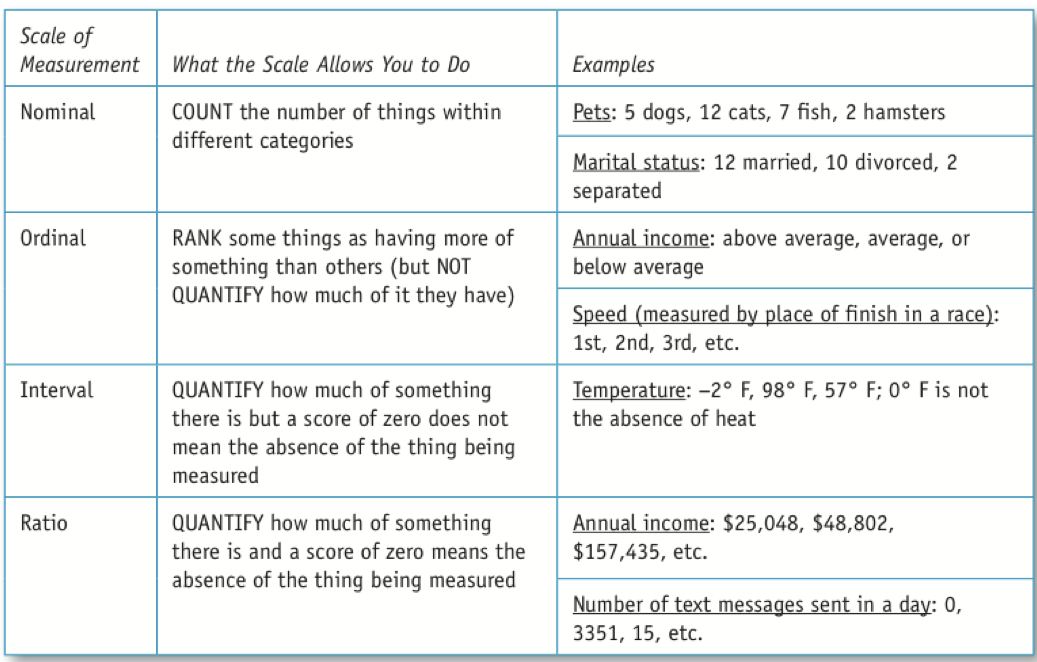
\includegraphics[width=0.8\linewidth]{figure/ExampleSOM}

\hypertarget{types-of-data-exercise}{%
\subsection{Types of Data (Exercise)}\label{types-of-data-exercise}}

State whether the variable is \textbf{continuous or discrete}, and
\textbf{quantitative or qualitative}.

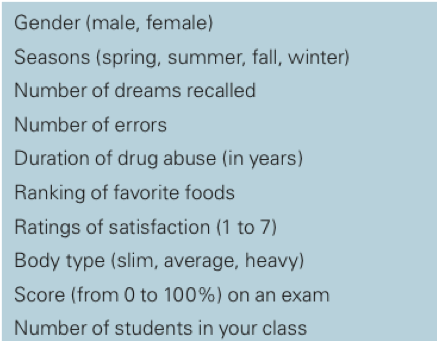
\includegraphics[width=0.4\linewidth]{figure/variables1}
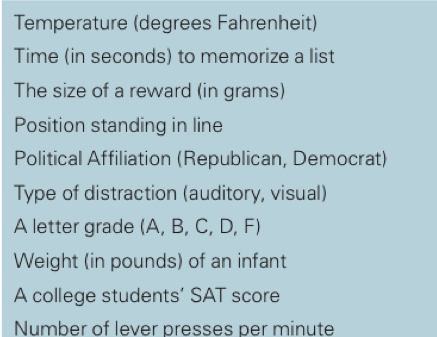
\includegraphics[width=0.4\linewidth]{figure/variables2}

\hypertarget{types-of-data-answer}{%
\subsection{Types of Data (Answer)}\label{types-of-data-answer}}

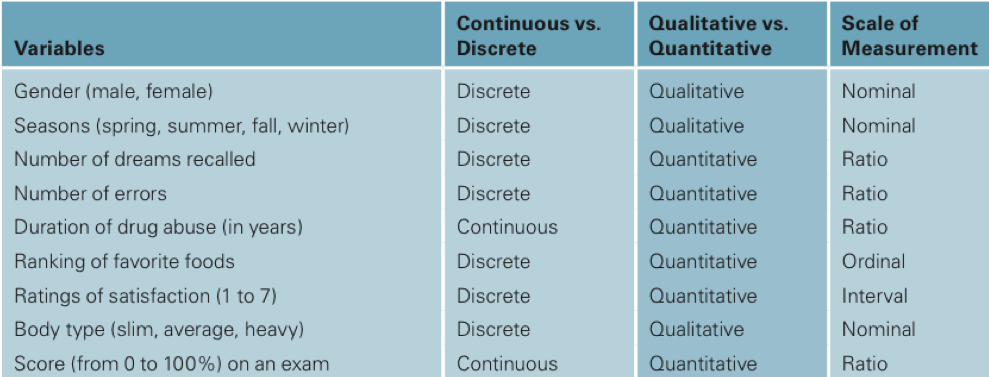
\includegraphics[width=0.9\linewidth,height=0.9\textheight]{figure/TOD1}

\hypertarget{types-of-data-cont.}{%
\subsection{Types of Data (cont.)}\label{types-of-data-cont.}}

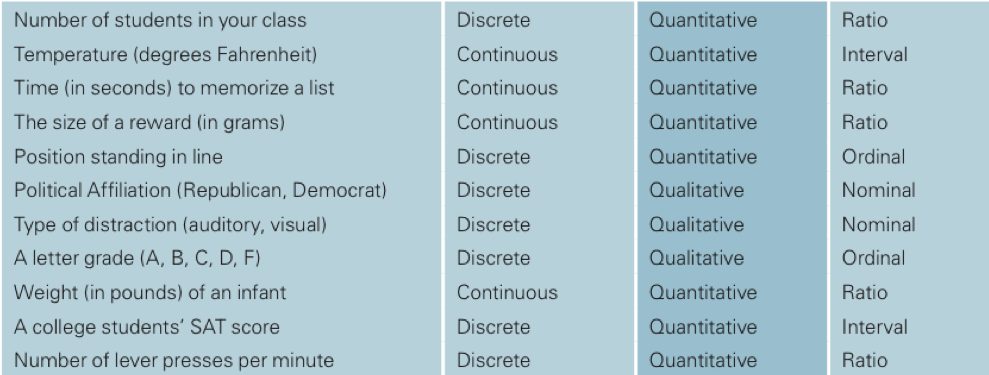
\includegraphics[width=0.9\linewidth,height=0.9\textheight]{figure/TOD2}

\hypertarget{exercises-types-of-variables}{%
\subsection{Exercises (Types of
Variables)}\label{exercises-types-of-variables}}

Name the \textbf{variable} being measured, (2) state whether it is
\textbf{continuous or discrete}, and (3) state whether the variable is
\textbf{quantitative or qualitative}.

\begin{enumerate}
\def\labelenumi{\arabic{enumi}.}
\tightlist
\item
  A researcher records the month of birth among patients with
  schizophrenia.
\item
  A professor records the number of students absent during final exam.
\item
  A researcher asks children to choose which type of cereal they prefer
  (one with a toy inside or one without). He records the choice of
  cereal.
\item
  A therapist measures the time (in hours) that clients continue a
  recommended program of counseling.
\end{enumerate}

\hypertarget{population-vs-sample}{%
\subsection{Population VS Sample}\label{population-vs-sample}}

\begin{itemize}
\tightlist
\item
  {\textbf{Population}} is a group of all things that share a set of
  characteristics.

  \begin{itemize}
  \tightlist
  \item
    Population parameter -- the value that would be obtained if the
    entire population were actually studied.
  \end{itemize}
\item
  {\textbf{Sample}} is a subset of population that is intended to
  represent the population.

  \begin{itemize}
  \tightlist
  \item
    Sample statistic -- the value obtained from the sample. It is used
    to estimate the population parameter value.
  \end{itemize}
\end{itemize}

\hypertarget{population-vs-sample-cont.}{%
\subsection{Population VS Sample
(cont.)}\label{population-vs-sample-cont.}}

\begin{itemize}
\tightlist
\item
  A set of data is a sample from our population. The sample is a subset
  of the population. Statistical inference -- the process that we used
  to draw conclusions from a data.
\item
  Inference involves using statistics we {\textbf{calculate from the
  sample to make and informed guess}} about population.
\item
  When we do statistical inference we are interested in drawing
  conclusions from a set of data (sample) so that we can estimate
  {\textbf{population parameters}}.
\end{itemize}

\hypertarget{statistical-inference}{%
\subsection{Statistical Inference}\label{statistical-inference}}

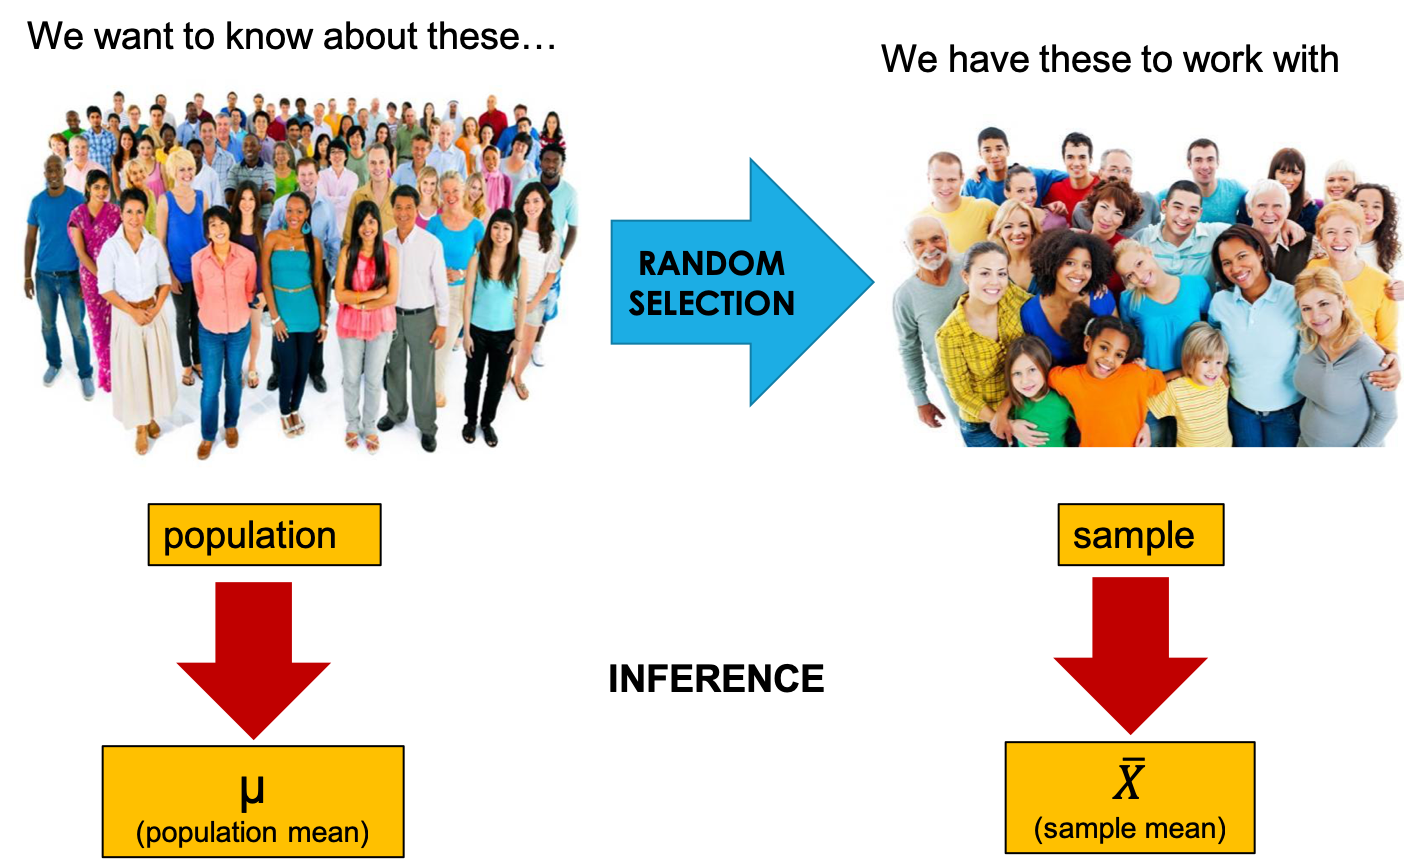
\includegraphics[width=0.8\linewidth]{figure/Ch1-SnP}

\hypertarget{population-vs-sample-cont.-1}{%
\subsection{Population VS Sample
(cont.)}\label{population-vs-sample-cont.-1}}

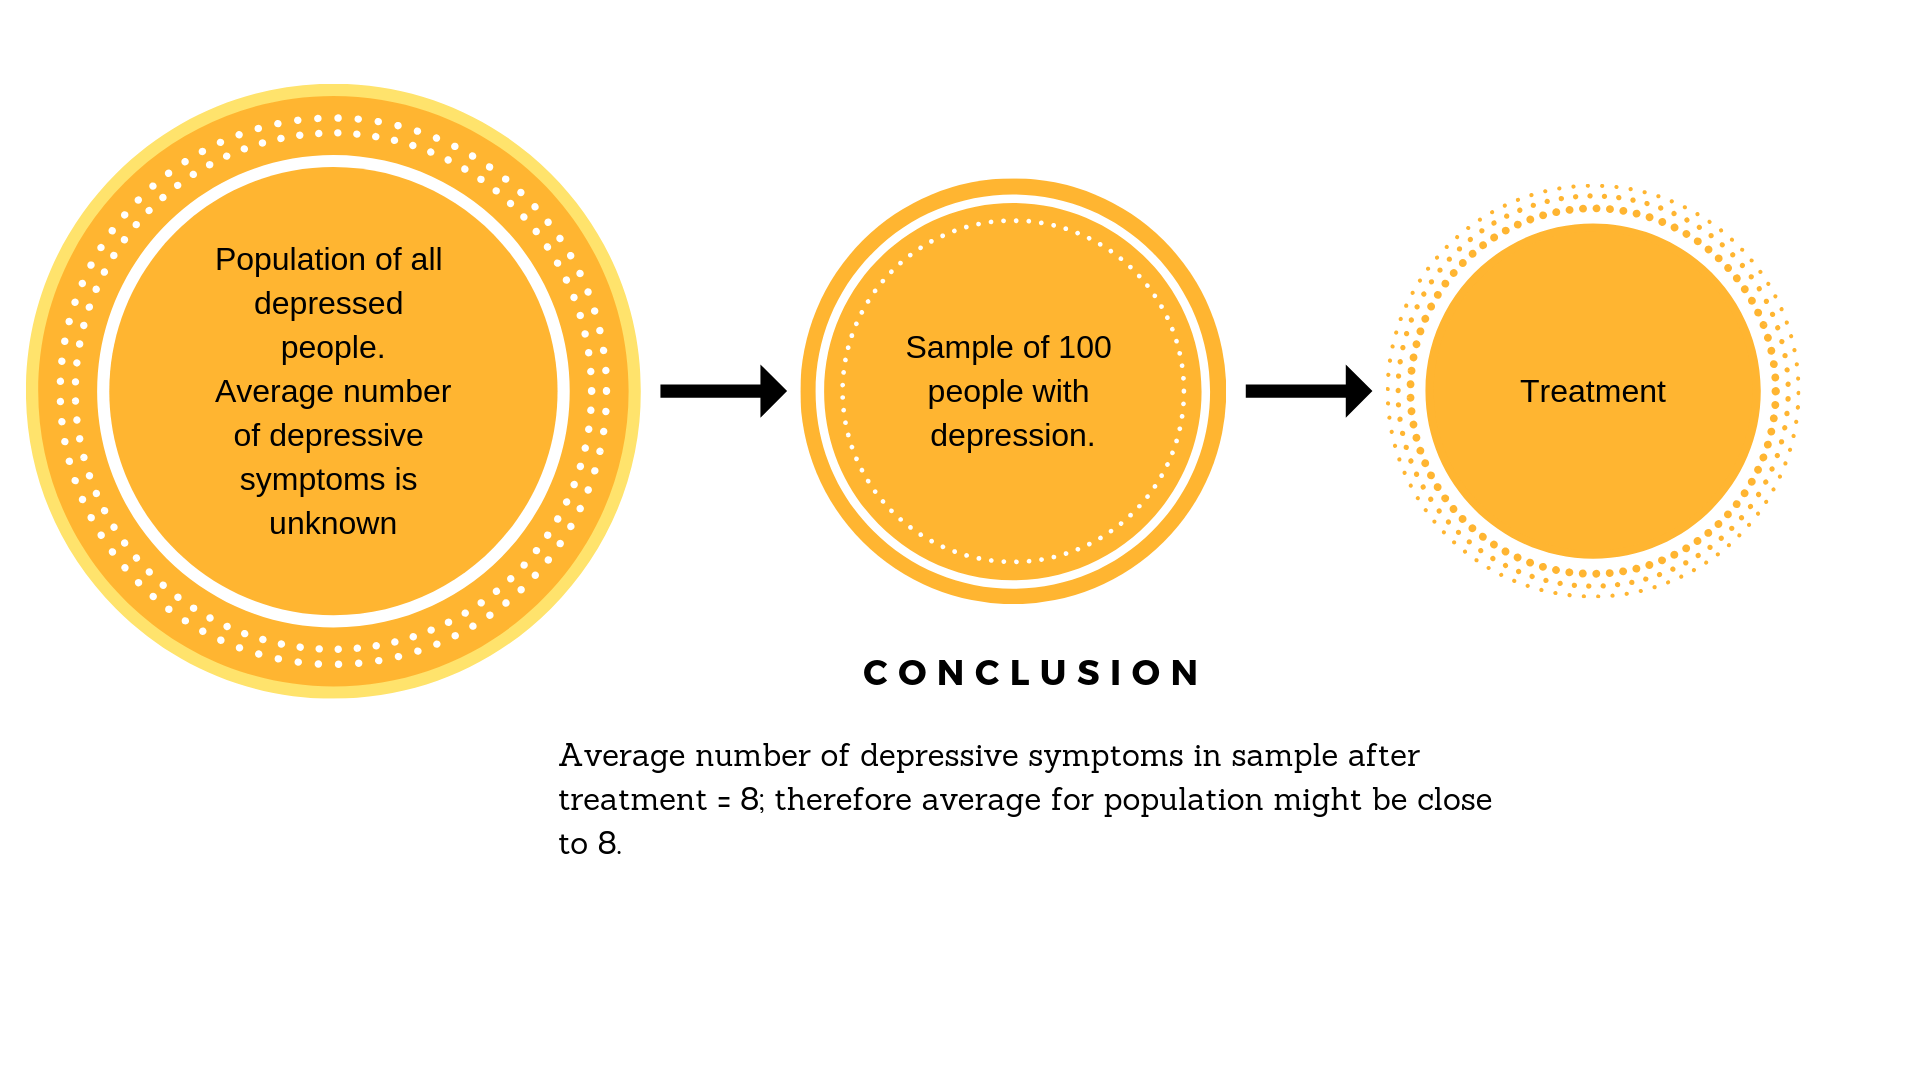
\includegraphics[width=1\linewidth]{figure/PopNSam}

\hypertarget{population-vs-sample-cont.-2}{%
\subsection{Population VS Sample
(cont.)}\label{population-vs-sample-cont.-2}}

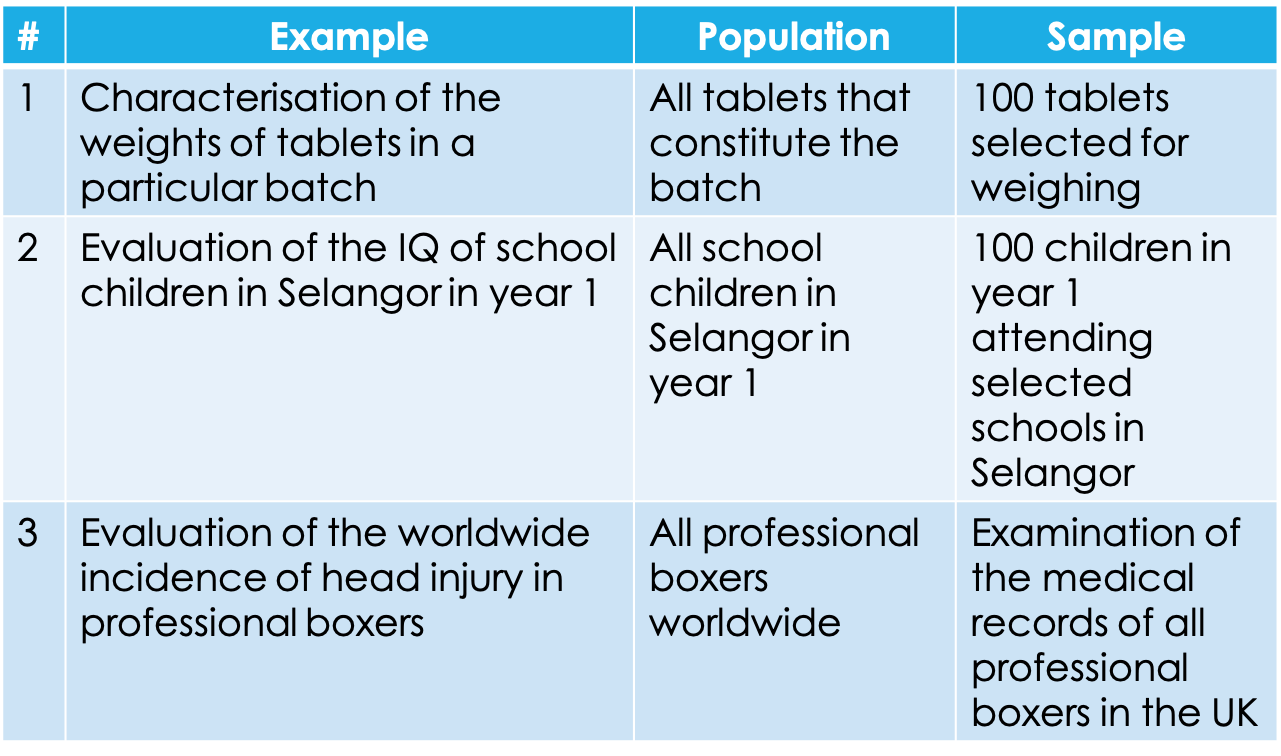
\includegraphics[width=0.8\linewidth]{figure/PopNSam2}

\hypertarget{describing-distributions}{%
\subsection{Describing Distributions}\label{describing-distributions}}

\begin{enumerate}
\def\labelenumi{\arabic{enumi}.}
\tightlist
\item
  Measures of Central Tendency
\item
  Measures of Dispersion
\end{enumerate}

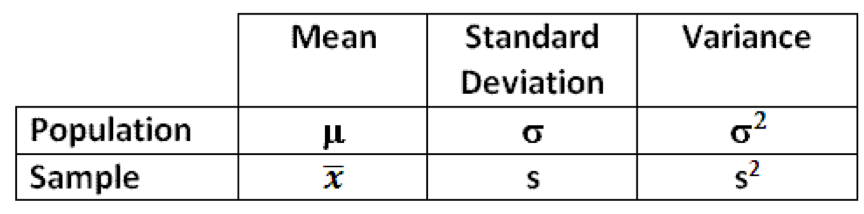
\includegraphics[width=0.95\linewidth]{figure/Ch1-symbols}

\hypertarget{measures-of-central-tendency}{%
\subsection{Measures of Central
Tendency}\label{measures-of-central-tendency}}

\begin{itemize}
\item
  Also known as {\textbf{measures of central location}} (locate central
  distribution).
\item
  {\textbf{Three kinds of averages of a data set}} to answer ``where do
  the data center?''
\item
  Measures include:

  \begin{enumerate}
  \def\labelenumi{\arabic{enumi}.}
  \tightlist
  \item
    Mean
  \item
    Mode
  \item
    Median
  \end{enumerate}
\end{itemize}

\hypertarget{the-mean}{%
\subsection{The Mean}\label{the-mean}}

\begin{itemize}
\tightlist
\item
  The usual ``average'' that is familiar to everyone.
\item
  Adds up all the numbers (\(\sum{X}\)) and divide by how many numbers
  there are (N for population or n for sample).
\item
  Formula:

  \begin{itemize}
  \tightlist
  \item
    Sample mean: \[\bar{X}=\frac{\sum_{i=1}^n X_i}{n}\]
  \item
    Population mean: \[\mu=\frac{\sum_{i=1}^N X_i}{N}\]
  \end{itemize}
\end{itemize}

\hypertarget{the-mean-example}{%
\subsection{The Mean (example)}\label{the-mean-example}}

The reduction in blood pressure (mmHg) in 6 patients 4 hours after
administration of a standard dose of a novel antihypertensive agent is
shown in Table 1.1. Calculate the mean reduction in blood pressure
reduction in the 6 patients.

\begin{table}

\caption{\label{tab:unnamed-chunk-10}Table 1.1 Effect of an antihypertensive drug on blood pressure lowering in six patients}
\centering
\fontsize{20}{22}\selectfont
\begin{tabular}[t]{c|c}
\hline
Patient number & Reduction in BP (mmHg)\\
\hline
1 & 20\\
\hline
2 & 25\\
\hline
3 & 21\\
\hline
4 & 34\\
\hline
5 & 31\\
\hline
6 & 37\\
\hline
\end{tabular}
\end{table}

\hypertarget{the-mean-example-1}{%
\subsection{The Mean (example)}\label{the-mean-example-1}}

\begin{itemize}
\tightlist
\item
  Substituting the figures from Table 1.1 into the equation for the
  mean, we obtain:
\end{itemize}

\[\begin{aligned} &= (20 + 25 + 21 + 34 + 41 + 37)/6 \\ &= 178/6 \\ &= 29.67   \end{aligned}\]

\hypertarget{the-weighted-mean}{%
\subsection{The Weighted Mean}\label{the-weighted-mean}}

\begin{itemize}
\tightlist
\item
  Each datum point in the distribution does not contribute equally to
  the overall calculation of the mean.
\item
  Data is divided into groups, each of which possesses different
  weighting.
\item
  Formula:\\
  \[\frac{\sum_{j=1}^N w_j X_j}{N}\]
\end{itemize}

\hypertarget{the-weighted-mean-example}{%
\subsection{The Weighted Mean
(Example)}\label{the-weighted-mean-example}}

The effect of a defined dose of a commercially available analgesic to
suppress pain following a painful stimulus was evaluated in 20
volunteers using an analogue scale (Table 1.2). Calculate the mean of
the pain assessment by the 20 volunteers.

\begin{table}

\caption{\label{tab:unnamed-chunk-11}Table 1.2 Recorded assessment of pain by 20 volunteers following administration of analgesic and exposure to a painful stimulus
}
\centering
\fontsize{20}{22}\selectfont
\begin{tabular}[t]{c|c}
\hline
Number of volunteers & Pain assessment by volunteers\\
\hline
2 & 3 (extreme pain)\\
\hline
12 & 2 (moderate pain)\\
\hline
6 & 1 (slight pain)\\
\hline
\end{tabular}
\end{table}

\hypertarget{the-weighted-mean-example-1}{%
\subsection{The Weighted Mean
(Example)}\label{the-weighted-mean-example-1}}

\begin{itemize}
\tightlist
\item
  Substituting the figures from Table 1.2 into the equation for the
  weighted arithmetic mean, we obtain:
\end{itemize}

\[\begin{aligned} &= (20 \times 3) + (12 \times 2) + (6 \times 1) / 20 \\ &= 36/20 \\ &= 1.8   \end{aligned}\]

\hypertarget{the-weighted-mean-frequency-distribution}{%
\subsection{The Weighted Mean (Frequency
Distribution)}\label{the-weighted-mean-frequency-distribution}}

\begin{table}[H]
\centering\begingroup\fontsize{20}{22}\selectfont

\begin{tabular}{c|c|c|c}
\hline
\rowcolor[HTML]{D7261E}  \begingroup\fontsize{20}{22}\selectfont \textcolor{white}{\textbf{Diameter (mm)}}\endgroup & \begingroup\fontsize{20}{22}\selectfont \textcolor{white}{\textbf{Frequency}}\endgroup & \begingroup\fontsize{20}{22}\selectfont \textcolor{white}{\textbf{Midpoint (x)}}\endgroup & \begingroup\fontsize{20}{22}\selectfont \textcolor{white}{\textbf{f.x}}\endgroup\\
\hline
35-39 & 6 & 37 & 222\\
\hline
40-44 & 12 & 42 & 504\\
\hline
45-49 & 15 & 47 & 705\\
\hline
50-54 & 10 & 52 & 520\\
\hline
55-59 & 7 & 57 & 399\\
\hline
Total & 50 &  & 2350\\
\hline
\end{tabular}
\endgroup{}
\end{table}

- Mean \(= 2350 / 50 = 47\)

\hypertarget{the-median}{%
\subsection{The Median}\label{the-median}}

\begin{itemize}
\tightlist
\item
  An alternative method of describing the central nature of data.
\item
  Relatively {\textbf{unaffected by the nature of the spread of data}}.
\item
  Is the middle number. It is found by putting the numbers in order and
  taking the actual middle number if there is one, or the average of the
  two middle numbers if not.
\end{itemize}

\hypertarget{the-median-example}{%
\subsection{The Median (Example)}\label{the-median-example}}

A random samples of yearly income of 7 employees (rounded to the nearest
hundred dollars):

\begin{table}[H]
\centering\begingroup\fontsize{22}{24}\selectfont

\begin{tabular}{>{\centering\arraybackslash}p{1.5cm}|>{\centering\arraybackslash}p{1.5cm}|>{\centering\arraybackslash}p{1.5cm}|>{\centering\arraybackslash}p{1.5cm}|>{\centering\arraybackslash}p{1.5cm}|>{\centering\arraybackslash}p{1.5cm}|>{\centering\arraybackslash}p{1.5cm}}
\hline
24.8 & 22.8 & 24.6 & 192.5 & 25.2 & 18.5 & 23.7\\
\hline
\end{tabular}
\endgroup{}
\end{table}

The mean (rounded in 1 decimal place is) : \textbf{47.4}, but the
statement {\textbf{the average income of 7 employees is \$47, 400}} is
certainly misleading.

\hypertarget{the-median-outliers}{%
\subsection{The Median (Outliers)}\label{the-median-outliers}}

\begin{table}[H]
\centering\begingroup\fontsize{25}{27}\selectfont

\begin{tabular}{>{\centering\arraybackslash}p{2cm}|>{\centering\arraybackslash}p{2cm}|>{\centering\arraybackslash}p{2cm}|>{\bfseries\leavevmode\color{white}\columncolor[HTML]{D7261E}}c|>{\centering\arraybackslash}p{2cm}|>{\centering\arraybackslash}p{2cm}|>{\centering\arraybackslash}p{2cm}}
\hline
24.8 & 22.8 & 24.6 & 192.5 & 25.2 & 18.5 & 23.7\\
\hline
\end{tabular}
\endgroup{}
\end{table}

\begin{itemize}
\tightlist
\item
  Number {\textbf{192.5}} is called outlier (far removed from most or
  all the remaining measurements).
\item
  Usually is the result of some sort of error (but not always).
\item
  Mean is sensitive to extreme values.
\item
  So, a better measure of the ``center'' of the data can be obtained if
  we were to arrange the data in numerical order.
\end{itemize}

\hypertarget{the-median-outliers-1}{%
\subsection{The Median (Outliers)}\label{the-median-outliers-1}}

\begin{itemize}
\tightlist
\item
  The order \textbackslash begin\{table\}{[}H{]}
  \centering\begingroup\fontsize{25}{27}\selectfont
\end{itemize}

\begin{tabular}{>{\centering\arraybackslash}p{2cm}|>{\centering\arraybackslash}p{2cm}|>{\centering\arraybackslash}p{2cm}|>{\bfseries\leavevmode\color{white}\columncolor[HTML]{581dd7}}c|>{\centering\arraybackslash}p{2cm}|>{\centering\arraybackslash}p{2cm}|>{\centering\arraybackslash}p{2cm}}
\hline
18.5 & 22.8 & 23.7 & 24.6 & 24.8 & 25.2 & 192.5\\
\hline
\end{tabular}
\endgroup{}

\textbackslash end\{table\}

\begin{itemize}
\tightlist
\item
  Then select the middle number in the list, in this case \textbf{24.6}.
\item
  In this sense, it locates the center of the data.
\end{itemize}

\hypertarget{the-median-outliers-2}{%
\subsection{The Median (Outliers)}\label{the-median-outliers-2}}

\begin{itemize}
\tightlist
\item
  If there are an even number of measurements in the data sets, there
  will be two middle elements -\textgreater{} take the mean of middle
  two as the median
\item
  Example: \textbackslash begin\{table\}{[}H{]}
  \centering\begingroup\fontsize{25}{27}\selectfont
\end{itemize}

\begin{tabular}{>{\centering\arraybackslash}p{2cm}|>{\centering\arraybackslash}p{2cm}|>{\centering\arraybackslash}p{2cm}|>{\bfseries\leavevmode\color[HTML]{581dd7}}c|>{\centering\arraybackslash}p{2cm}|>{\centering\arraybackslash}p{2cm}|>{\centering\arraybackslash}p{2cm}|>{\centering\arraybackslash}p{2cm}}
\hline
18.5 & 22.8 & 23.7 & 24.6 & 24.8 & 25.2 & 28.9 & 192.5\\
\hline
\end{tabular}
\endgroup{}

\textbackslash end\{table\}

\begin{itemize}
\tightlist
\item
  Median: (24.6 + 24.8) / 2 = 24.7
\end{itemize}

\hypertarget{the-mode}{%
\subsection{The Mode}\label{the-mode}}

\begin{itemize}
\tightlist
\item
  The easiest measure of the average.
\item
  Defined as the item of data with {\textbf{the highest frequency.}}
\item
  {\textbf{Most frequently occurring}} number.
\item
  For any data set there is always exactly one mean and exactly one
  median.
\item
  However, several different values could occur with the highest
  frequency.
\end{itemize}

\hypertarget{the-mode-cont.}{%
\subsection{The Mode (cont.)}\label{the-mode-cont.}}

\begin{itemize}
\item
  Data set 1: NA 
\item
  The mode of this data set is \textbf{0}.
\item
  Data set 2: NA 
\item
  Two most frequently observed values in this data set are 1 and 2.
  Therefore mode is a set of two values : {\textbf{\{1,2\}}}
\end{itemize}

\hypertarget{the-mode-median-and-mean-example}{%
\subsection{The Mode, Median and Mean
(Example)}\label{the-mode-median-and-mean-example}}

Weight of luggage presented by airline passengers at check-in (measured
to the nearest kg).

NA

Calculate \textbf{mode},\textbf{median} and \textbf{mean}.

\begin{itemize}
\item
  Mode: \textbf{20}
\item
  Median: \textbf{20}

  \begin{itemize}
  \tightlist
  \item
    put the numbers in order first and take the actual middle number
    (odd count) or the average middle number (even count). 
  \end{itemize}
\end{itemize}

\begin{table}[H]
\centering\begingroup\fontsize{25}{27}\selectfont

\begin{tabular}{>{\centering\arraybackslash}p{2cm}|>{\centering\arraybackslash}p{2cm}|>{\centering\arraybackslash}p{2cm}|>{\centering\arraybackslash}p{2cm}|>{\centering\arraybackslash}p{2cm}|>{\bfseries\leavevmode\color[HTML]{581dd7}}c|>{\centering\arraybackslash}p{2cm}|>{\centering\arraybackslash}p{2cm}|>{\centering\arraybackslash}p{2cm}|>{\centering\arraybackslash}p{2cm}|>{\centering\arraybackslash}p{2cm}}
\hline
15 & 18 & 19 & 20 & 20 & 20 & 21 & 23 & 23 & 24 & 24\\
\hline
\end{tabular}
\endgroup{}
\end{table}

- Mean = (15+18+19+20+20+20+21+23+23+24+24) / 11 = \textbf{20.64}

\hypertarget{when-not-to-use-the-mean}{%
\subsection{When not to use the mean?}\label{when-not-to-use-the-mean}}

\begin{itemize}
\tightlist
\item
  Mean is good for dataset that is evenly spread.
\item
  For normally distributed data, the numerical values of the mean and
  median should be identical and either term may successfully be used to
  describe the central point.
\item
  The use of median is preferable for distributions that possess extreme
  values (mean is unacceptably distorted). 
\end{itemize}

\begin{table}[H]
\centering\begingroup\fontsize{25}{27}\selectfont

\begin{tabular}{>{\raggedright\arraybackslash}p{2cm}|>{\centering\arraybackslash}p{2cm}|>{\centering\arraybackslash}p{2cm}|>{\centering\arraybackslash}p{2cm}|>{\centering\arraybackslash}p{2cm}|>{\centering\arraybackslash}p{2cm}|>{\centering\arraybackslash}p{2cm}|>{\centering\arraybackslash}p{2cm}|>{\centering\arraybackslash}p{2cm}|>{\centering\arraybackslash}p{2cm}|c}
\hline
Staff & 1 & 2 & 3 & 4 & 5 & 6 & 7 & 8 & 9 & 10\\
\hline
Salary & 15k & 18k & 16k & 14k & 15k & 15k & 12k & 17k & 90k & 95k\\
\hline
\end{tabular}
\endgroup{}
\end{table}

- The mean salary is \textbf{30.7k}

\hypertarget{measures-of-dispersion}{%
\subsection{Measures of Dispersion}\label{measures-of-dispersion}}

\begin{itemize}
\item
  Also known as {\textbf{measures of variation}}
\item
  How spread out are the data?
\item
  Describing quantitative data will not be complete without knowing how
  observed values are spread out from the average.
\item
  E.g: two classes who sat the same exam might have the same mean mark
  but the marks may vary in a different pattern around this.
\item
  Measures include:

  \begin{enumerate}
  \def\labelenumi{\arabic{enumi}.}
  \tightlist
  \item
    Range
  \item
    Variance
  \item
    Standard Deviation (SD)
  \end{enumerate}
\end{itemize}

\hypertarget{measures-of-dispersion-example}{%
\subsection{Measures of Dispersion
(Example)}\label{measures-of-dispersion-example}}

\begin{itemize}
\tightlist
\item
  Example:\\
  \textbackslash begin\{table\}
\end{itemize}

\caption{\label{tab:unnamed-chunk-22}Table 1.3: Individual values associated with two sets of data possessing identical means.}
\centering
\begin{tabu} to \linewidth {>{\centering}X>{\centering}X}
\hline
\rowcolor[HTML]{D7261E}  \begingroup\fontsize{24}{26}\selectfont \textcolor{white}{\textbf{Set A}}\endgroup & \begingroup\fontsize{24}{26}\selectfont \textcolor{white}{\textbf{Set B}}\endgroup\\
\hline
10 & \vphantom{1} 28\\
\hline
20 & \vphantom{1} 29\\
\hline
30 & 30\\
\hline
20 & 29\\
\hline
10 & 28\\
\hline
**Mean: 30** & **Mean: 30**\\
\hline
\end{tabu}

\textbackslash end\{table\}

\hypertarget{range}{%
\subsection{Range}\label{range}}

\begin{itemize}
\item
  Very simple measure of dispersion.
\item
  Difference between the maximum value and the minimum value (max-min).
\item
  Example

  \begin{enumerate}
  \def\labelenumi{\arabic{enumi}.}
  \tightlist
  \item
    Marks on test A
  \end{enumerate}

  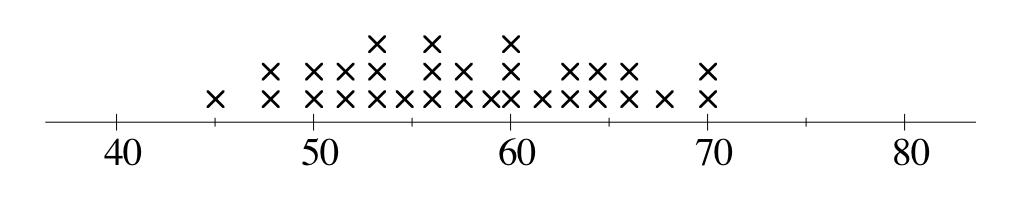
\includegraphics[width=0.8\linewidth]{figure/testA-range}

  \begin{enumerate}
  \def\labelenumi{\arabic{enumi}.}
  \setcounter{enumi}{1}
  \tightlist
  \item
    Marks on test B
  \end{enumerate}

  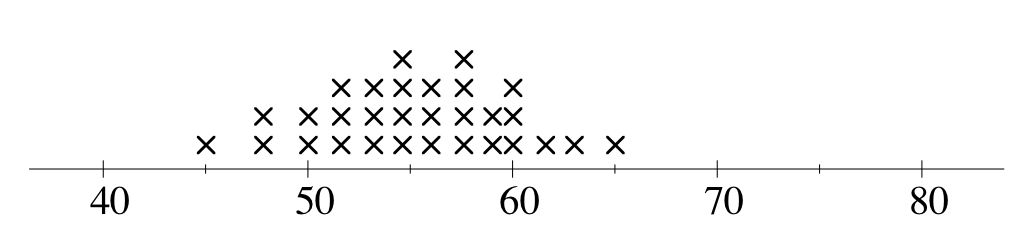
\includegraphics[width=0.8\linewidth]{figure/testB-range}
\end{itemize}

\hypertarget{range-calculation}{%
\subsection{Range Calculation}\label{range-calculation}}

\begin{enumerate}
\def\labelenumi{\arabic{enumi}.}
\tightlist
\item
  Marks on test A

  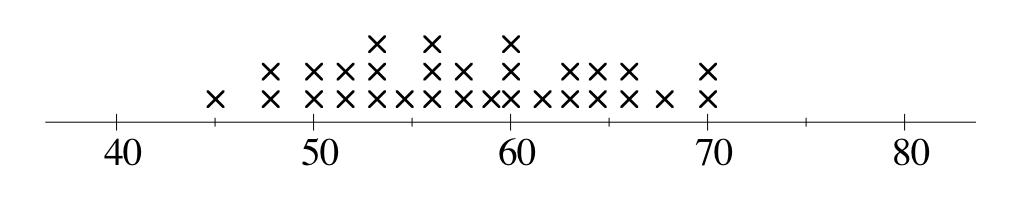
\includegraphics[width=0.8\linewidth]{figure/testA-range}
\end{enumerate}

\begin{enumerate}
\def\labelenumi{\arabic{enumi}.}
\setcounter{enumi}{1}
\tightlist
\item
  Marks on test B

  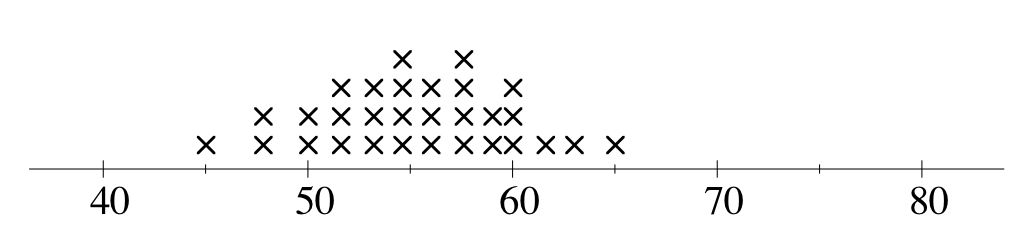
\includegraphics[width=0.8\linewidth]{figure/testB-range}
\end{enumerate}

On test A, the range of marks is \textbf{70-45=25}. On test B, the range
of marks is \textbf{65-45=20}.

\hypertarget{range-another-example}{%
\subsection{Range (another example)}\label{range-another-example}}

\begin{enumerate}
\def\labelenumi{\arabic{enumi}.}
\setcounter{enumi}{2}
\tightlist
\item
  Marks on test C

  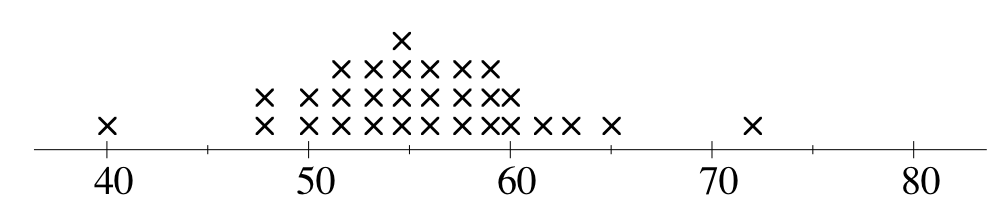
\includegraphics[width=0.8\linewidth]{figure/testC-range}
\end{enumerate}

\begin{itemize}
\tightlist
\item
  On test C, the range of marks is \textbf{75-40=32}.
\end{itemize}

\hypertarget{variance}{%
\subsection{Variance}\label{variance}}

\begin{itemize}
\tightlist
\item
  Squared deviations from the mean.
\item
  The sample variance of a set of n sample data is the number (\(s^2\))
  defined by the formula: \[s^2=\frac{\sum(X-\bar{X})^2}{n-1}\]
\item
  The population variance (\(\sigma^2\)) formula :
  \[\sigma^2=\frac{\sum(X-\mu)^2}{N}\]
\end{itemize}

\hypertarget{standard-deviation}{%
\subsection{Standard Deviation}\label{standard-deviation}}

\begin{itemize}
\tightlist
\item
  Measure of variation (deviation) of all values from the mean.
\item
  Positive square root of the variance.
\item
  Properties include:

  \begin{itemize}
  \tightlist
  \item
    The value is usually positive.
  \item
    0 indicates no variation.
  \item
    Larger values indicate greater variation.
  \item
    The value can increase dramatically with the inclusion of one or
    more outliers.
  \item
    The units are the same as the units of the original data values.
  \end{itemize}
\end{itemize}

\hypertarget{standard-deviation-formula}{%
\subsection{Standard Deviation
(formula)}\label{standard-deviation-formula}}

\begin{itemize}
\tightlist
\item
  Sample standard deviation formula
  \[s=\sqrt\frac{\sum(X-\bar{X})^2}{n-1}\]
\item
  The population standard deviation formula
  \[\sigma=\sqrt{\sigma^2}=\sqrt\frac{\sum(X-\mu)^2}{N}\]
\end{itemize}

\hypertarget{procedure-for-finding-the-standard-deviation-sample}{%
\subsection{Procedure for finding the standard deviation
(sample)}\label{procedure-for-finding-the-standard-deviation-sample}}

\begin{enumerate}
\def\labelenumi{\arabic{enumi}.}
\tightlist
\item
  Compute the mean (\(\bar{X}\))
\item
  Subtract the mean from each individual value to get a list of
  deviations of the form: (\(X – \bar{X}\))
\item
  Square each of the differences obtained from step 2:
  \((X – \bar{X})^2\)
\item
  Add all of the squares obtained from step 3: \(\sum(X – \bar{X})^2\)
\item
  Divide the total from step 4 by the number (n -- 1), which is 1 less
  than the total number of values present:
  \(\frac{\sum(X – \bar{X})^2}{n-1}\)
\item
  Find the square root of the result of step 5:
  \(\sqrt{\frac{\sum(X – \bar{X})^2}{n-1}}\)
\end{enumerate}

\hypertarget{standard-deviation-example}{%
\subsection{Standard Deviation
(Example)}\label{standard-deviation-example}}

\begin{itemize}
\tightlist
\item
  Multiple waiting line: 1, 3, 4
\item
  Compute the mean (\(\bar{X}\)) = 18 / 3 = 6 min 
\end{itemize}

\begin{tabu} to \linewidth {>{\centering}X>{\centering}X>{\centering}X}
\hline
\rowcolor[HTML]{D7261E}  \begingroup\fontsize{24}{26}\selectfont \textcolor{white}{\textbf{\$X\$}}\endgroup & \begingroup\fontsize{24}{26}\selectfont \textcolor{white}{\textbf{\$X-mean\$}}\endgroup & \begingroup\fontsize{24}{26}\selectfont \textcolor{white}{\textbf{\$X-mean\textasciicircum{}2\$}}\endgroup\\
\hline
1 & -5 & 25\\
\hline
3 & -3 & 9\\
\hline
14 & 8 & 64\\
\hline
**18** &  & **98**\\
\hline
\end{tabu}

\begin{itemize}
\tightlist
\item
  Variance: 98 / 2 = 49
\item
  Standard deviation: \(\sqrt{49}\) = \textbf{7.0 min}
\end{itemize}

\hypertarget{describing-distribution}{%
\subsection{Describing Distribution}\label{describing-distribution}}

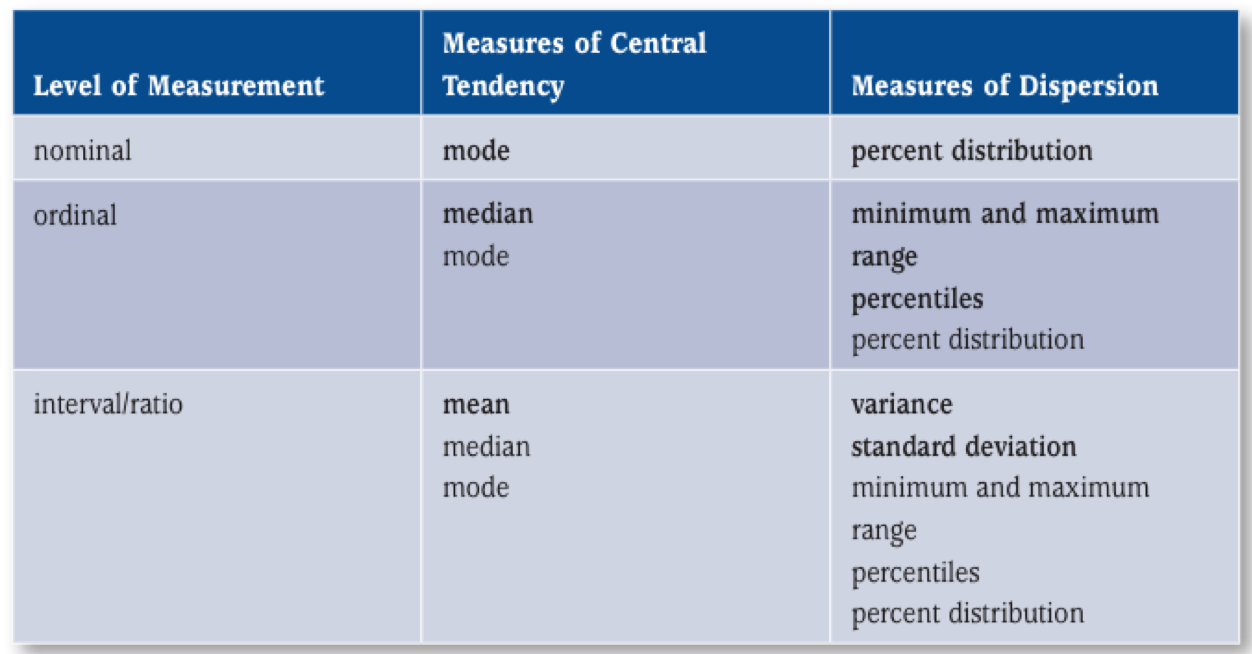
\includegraphics[width=0.8\linewidth]{figure/distribution}

\hypertarget{range-rule-of-thumb}{%
\subsection{Range Rule of Thumb}\label{range-rule-of-thumb}}

\begin{itemize}
\item
  For interpreting a known value of the standard deviation

  \begin{enumerate}
  \def\labelenumi{\arabic{enumi}.}
  \tightlist
  \item
    Minimum ``usual'' value = (mean) -- 2 x standard deviation
  \item
    Maximum ``usual'' value = (mean) + 2 x standard deviation
  \end{enumerate}
\end{itemize}

\hypertarget{rule-of-thumb-example}{%
\subsection{Rule of Thumb (Example)}\label{rule-of-thumb-example}}

Past results from the National Health Survey suggest that the head
circumferences of 2 months old girls have a {\textbf{mean of 40.05}} cm
and a {\textbf{standard deviation of 1.64}} cm. Determine whether a
circumference of 42.6 cm would be considered ``unusual''.

\hypertarget{rule-of-thumb-solution}{%
\subsection{Rule of Thumb (Solution)}\label{rule-of-thumb-solution}}

\begin{itemize}
\tightlist
\item
  With a mean of 40.05 cm and a standard deviation of 1.64 cm, we use
  the range rule of thumb to find the minimum and maximum usual
  circumferences as follows:

  \begin{enumerate}
  \def\labelenumi{\arabic{enumi}.}
  \tightlist
  \item
    Minimum usual value = (mean) -- 2 x (standard deviation) = 40.05 --
    2 x 1.64 = \textbf{36.77 cm}
  \item
    Maximum usual value = (mean) + 2 x (standard deviation) = 40.05 + 2
    x 1.64 = \textbf{43.33 cm}
  \end{enumerate}
\item
  Based on these results, we expect that typical two-month-old girls
  have head circumferences between 36.77 cm and 43.33 cm.
\item
  Because 42.6 cm falls within those limits, it would be considered
  usual or typical, not unusual.
\end{itemize}

\hypertarget{skewness}{%
\subsection{Skewness}\label{skewness}}

\begin{itemize}
\tightlist
\item
  Skewness

  \begin{itemize}
  \tightlist
  \item
    Refer to shape of distribution, either symmetry or assymetry
  \end{itemize}
\item
  Kurtosis

  \begin{itemize}
  \tightlist
  \item
    Refer to the flatness or peakness of a distribution
  \end{itemize}
\end{itemize}

\hypertarget{positively-skewed-distribution}{%
\subsection{Positively Skewed
Distribution}\label{positively-skewed-distribution}}

\begin{itemize}
\tightlist
\item
  Tail pointing to the larger value
\item
  Mean \textgreater{} Median \textgreater{} Mode

  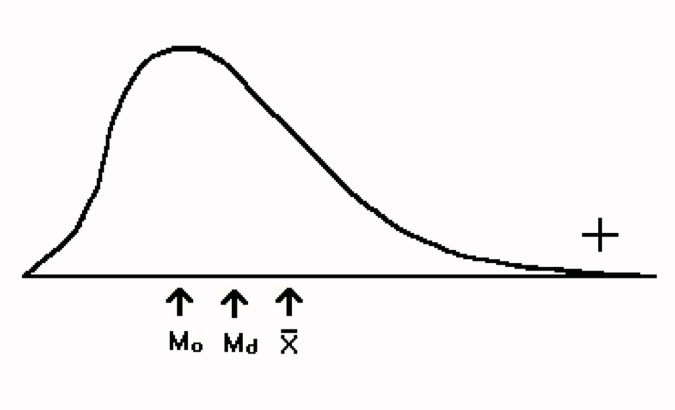
\includegraphics[width=0.8\linewidth]{figure/positive-skew}
\end{itemize}

\hypertarget{negatively-skewed-distribution}{%
\subsection{Negatively Skewed
Distribution}\label{negatively-skewed-distribution}}

\begin{itemize}
\tightlist
\item
  Tail pointing to the smaller value
\item
  Mode \textgreater{} Median \textgreater{} Mean

  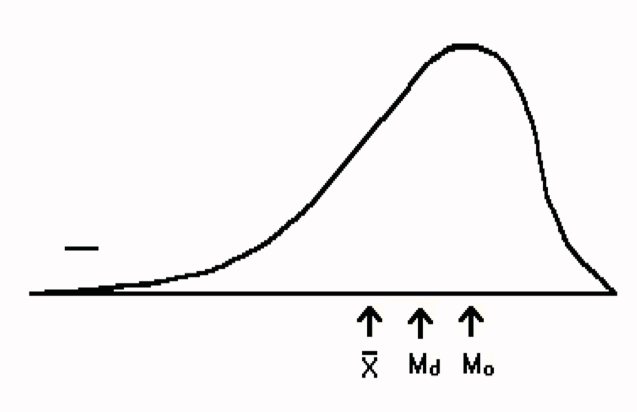
\includegraphics[width=0.8\linewidth]{figure/negative-skew}
\end{itemize}

\hypertarget{kurtosis}{%
\subsection{Kurtosis}\label{kurtosis}}

\begin{itemize}
\item
  Platykurtic distribution

  \begin{itemize}
  \tightlist
  \item
    Low peak
  \item
    Flatter than the normal curve
  \end{itemize}
\item
  Leptokurtic distribution

  \begin{itemize}
  \tightlist
  \item
    High peak
  \item
    More peaked than the normal curve
  \end{itemize}

  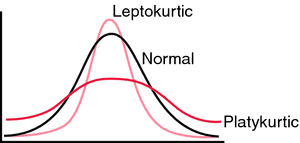
\includegraphics[width=0.8\linewidth]{figure/kurtosis}
\end{itemize}

\hypertarget{section}{%
\subsection{}\label{section}}

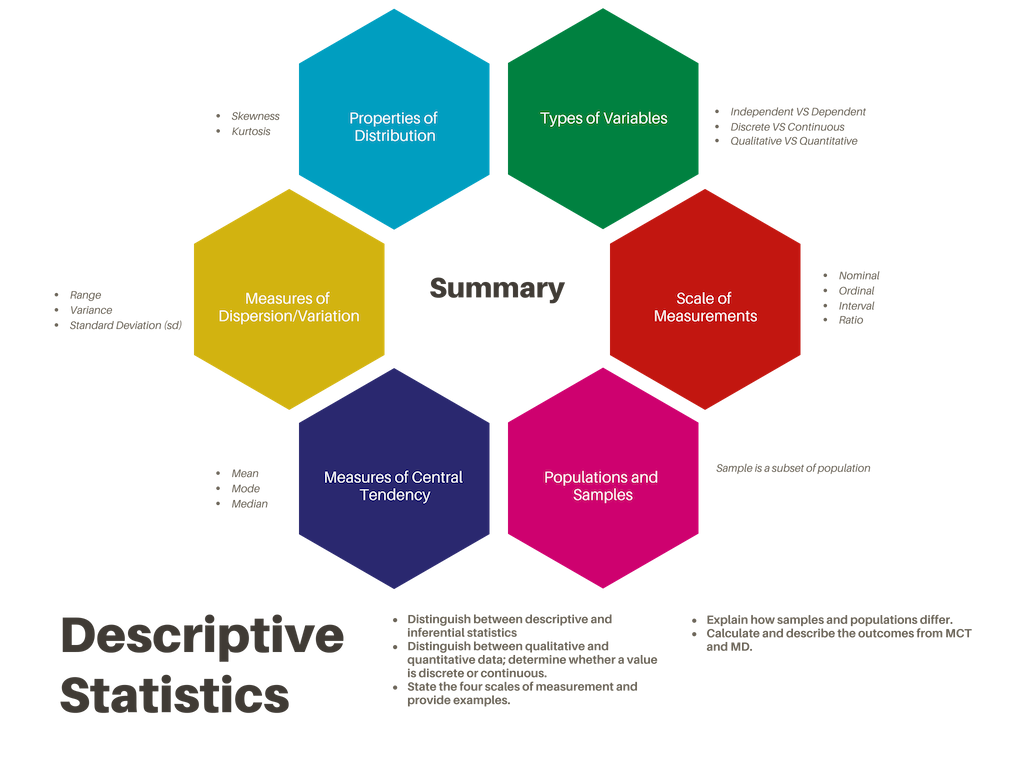
\includegraphics[width=0.85\linewidth]{figure/summary-Trans}


\end{document}
